\documentclass{beamer}
\usetheme{metropolis}           % Use metropolis theme
\usepackage[utf8]{inputenc}
\usepackage[brazil]{babel}
\usepackage[normalem]{ulem}
\usepackage{float}
\usepackage{caption}
\usepackage{subcaption}
\usepackage[style = abnt, backend = biber]{biblatex}
\addbibresource{refs.bib}
\title{Emergência de distribuições de posicionamentos ideológicos: uma abordagem
computacional}
\date{}
\author{Marcelo Veloso Maciel}
\institute{}
\begin{document}
\maketitle



% ----------------- NOVO SLIDE --------------------------------
\begin{frame}{Sumário}
\tableofcontents
\end{frame}



\section{Introdução}
\begin{frame}{Objetivo}
  Propor e analisar um modelo generativo de Opinião Pública
\end{frame}


\begin{frame}{Justificativa}
  \begin{itemize}
  \item Normativa
  \item Positiva: 
  \begin{itemize}
  \item Modelagem Baseada em Agentes;
    \item Emergência;
  \end{itemize}
  \end{itemize}
\end{frame}

\begin{frame}{Escopo}
  \begin{itemize}
  \item Sistema Alvo \(\rightarrow\) ``Opiniões Públicas Nacionais''
  \item Microfundamentos da Opinião Pública = Opinião Idiossincrática +
    Influência Social (Pares e \sout{Mídia} )
  \end{itemize}
  
\end{frame}

\section{Fundamentação Teórica}
\begin{frame}{Literaturas}

Critérios de Fidelidade \cite{weisberg2012simulation}:
\begin{itemize}
\item Estrutura;
\item \textit{Output}.
\end{itemize}
  
Base para a construção do modelo:

\begin{itemize}
\item Teoria Política Formal
\item Dinâmicas de Opinião
\item \textcolor{gray!70}{Opinião Pública}
\end{itemize}
\end{frame}

\begin{frame}{Teoria Política Formal}

  \begin{itemize}
  \item Modelagem Formal de Política;
  \item Principal subconjunto: Teoria da Escolha Racional;
  \item Modelo do ator racional: Preferências e Crenças Consistentes + Atualização
    Bayesiana.
  \end{itemize}

\end{frame}


\begin{frame}{Teoria Espacial e Eleições: Microfundamentos I}
  \begin{itemize}
  \item Teoria Política Espacial : analogia espacial;
  \item Comitês x Eleições de Larga Escala;
  \item Atitudes e  Ideologia.
  \end{itemize}
\end{frame}

\begin{frame}{Teoria Espacial e Eleições: Macrofundamentos I }
  \begin{itemize}
\item \textcite{druckman2012public} aponta dois achados canônicos da Opinião
  Pública:
  \begin{itemize}
  \item Instabilidade Micro;
  \item Estabilidade Macro.
  \end{itemize}
  \end{itemize}
  
\end{frame}


\begin{frame}{Teoria Espacial e Eleições: Macrofundamentos I }
  \begin{figure}[H]
    \centering
    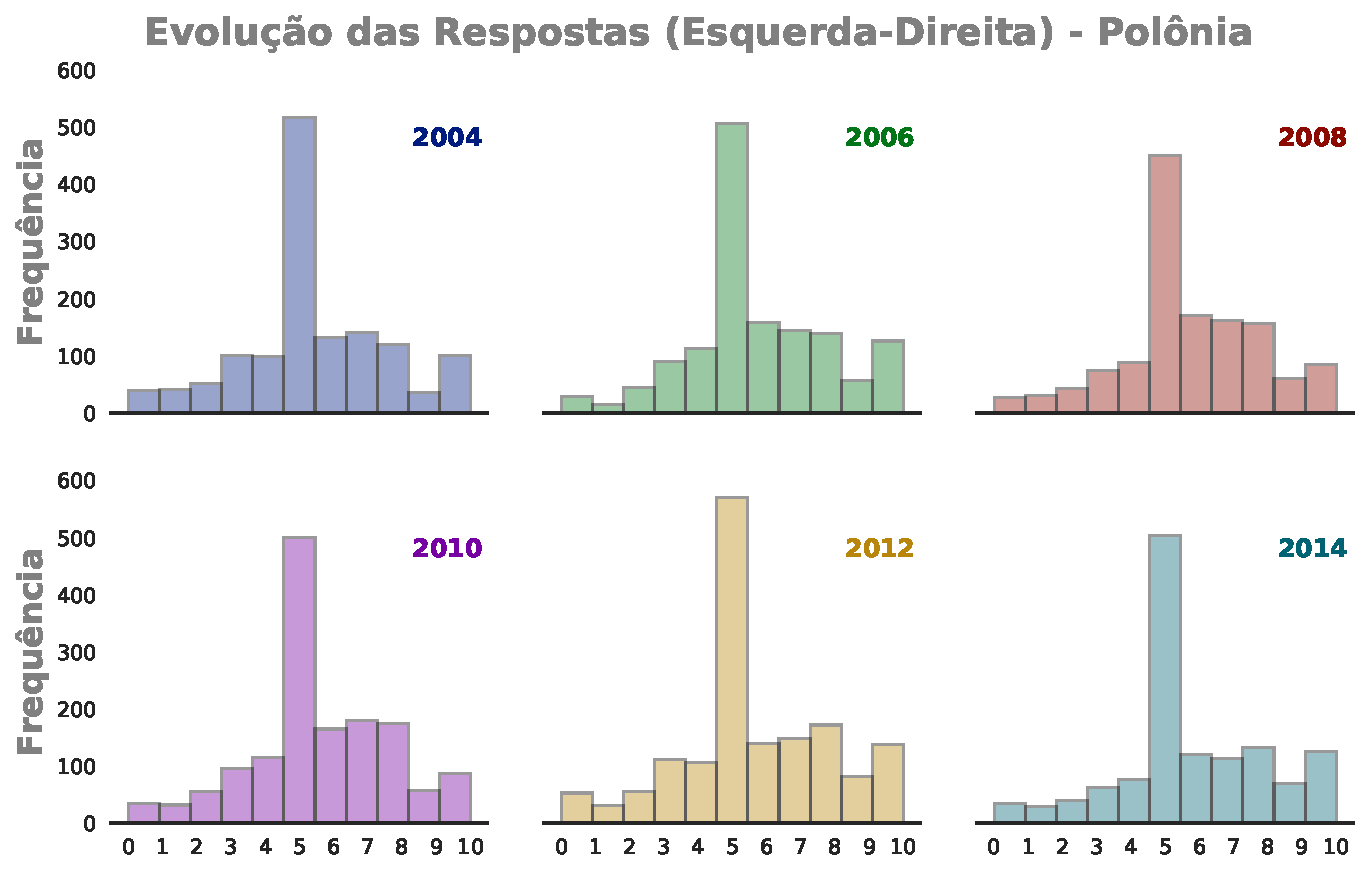
\includegraphics[scale = 0.4]{ims/ess_Pol_plots.pdf}
    \caption{Estabilidade Ideológica}
    \label{fig1}
  \end{figure}
\end{frame}


\begin{frame}{Teoria Espacial e Eleições: Macrofundamentos II}

  \begin{itemize}
 \item \textcite{flache2017} aponta os seguintes fatos estilizados sobre
   distribuições de opinião pública no ESS:
    \begin{itemize}
    \item  há um pico central dominante;
    \item há uma tendência para a existência de \textit{clusters} não centrais;
    \item há uma tendência a picos nos extremos.
    \end{itemize}
  \end{itemize}
  
\end{frame}

\begin{frame}{Teoria Espacial e Eleições: Macrofundamentos II}  
  \begin{figure}[H]
      \centering 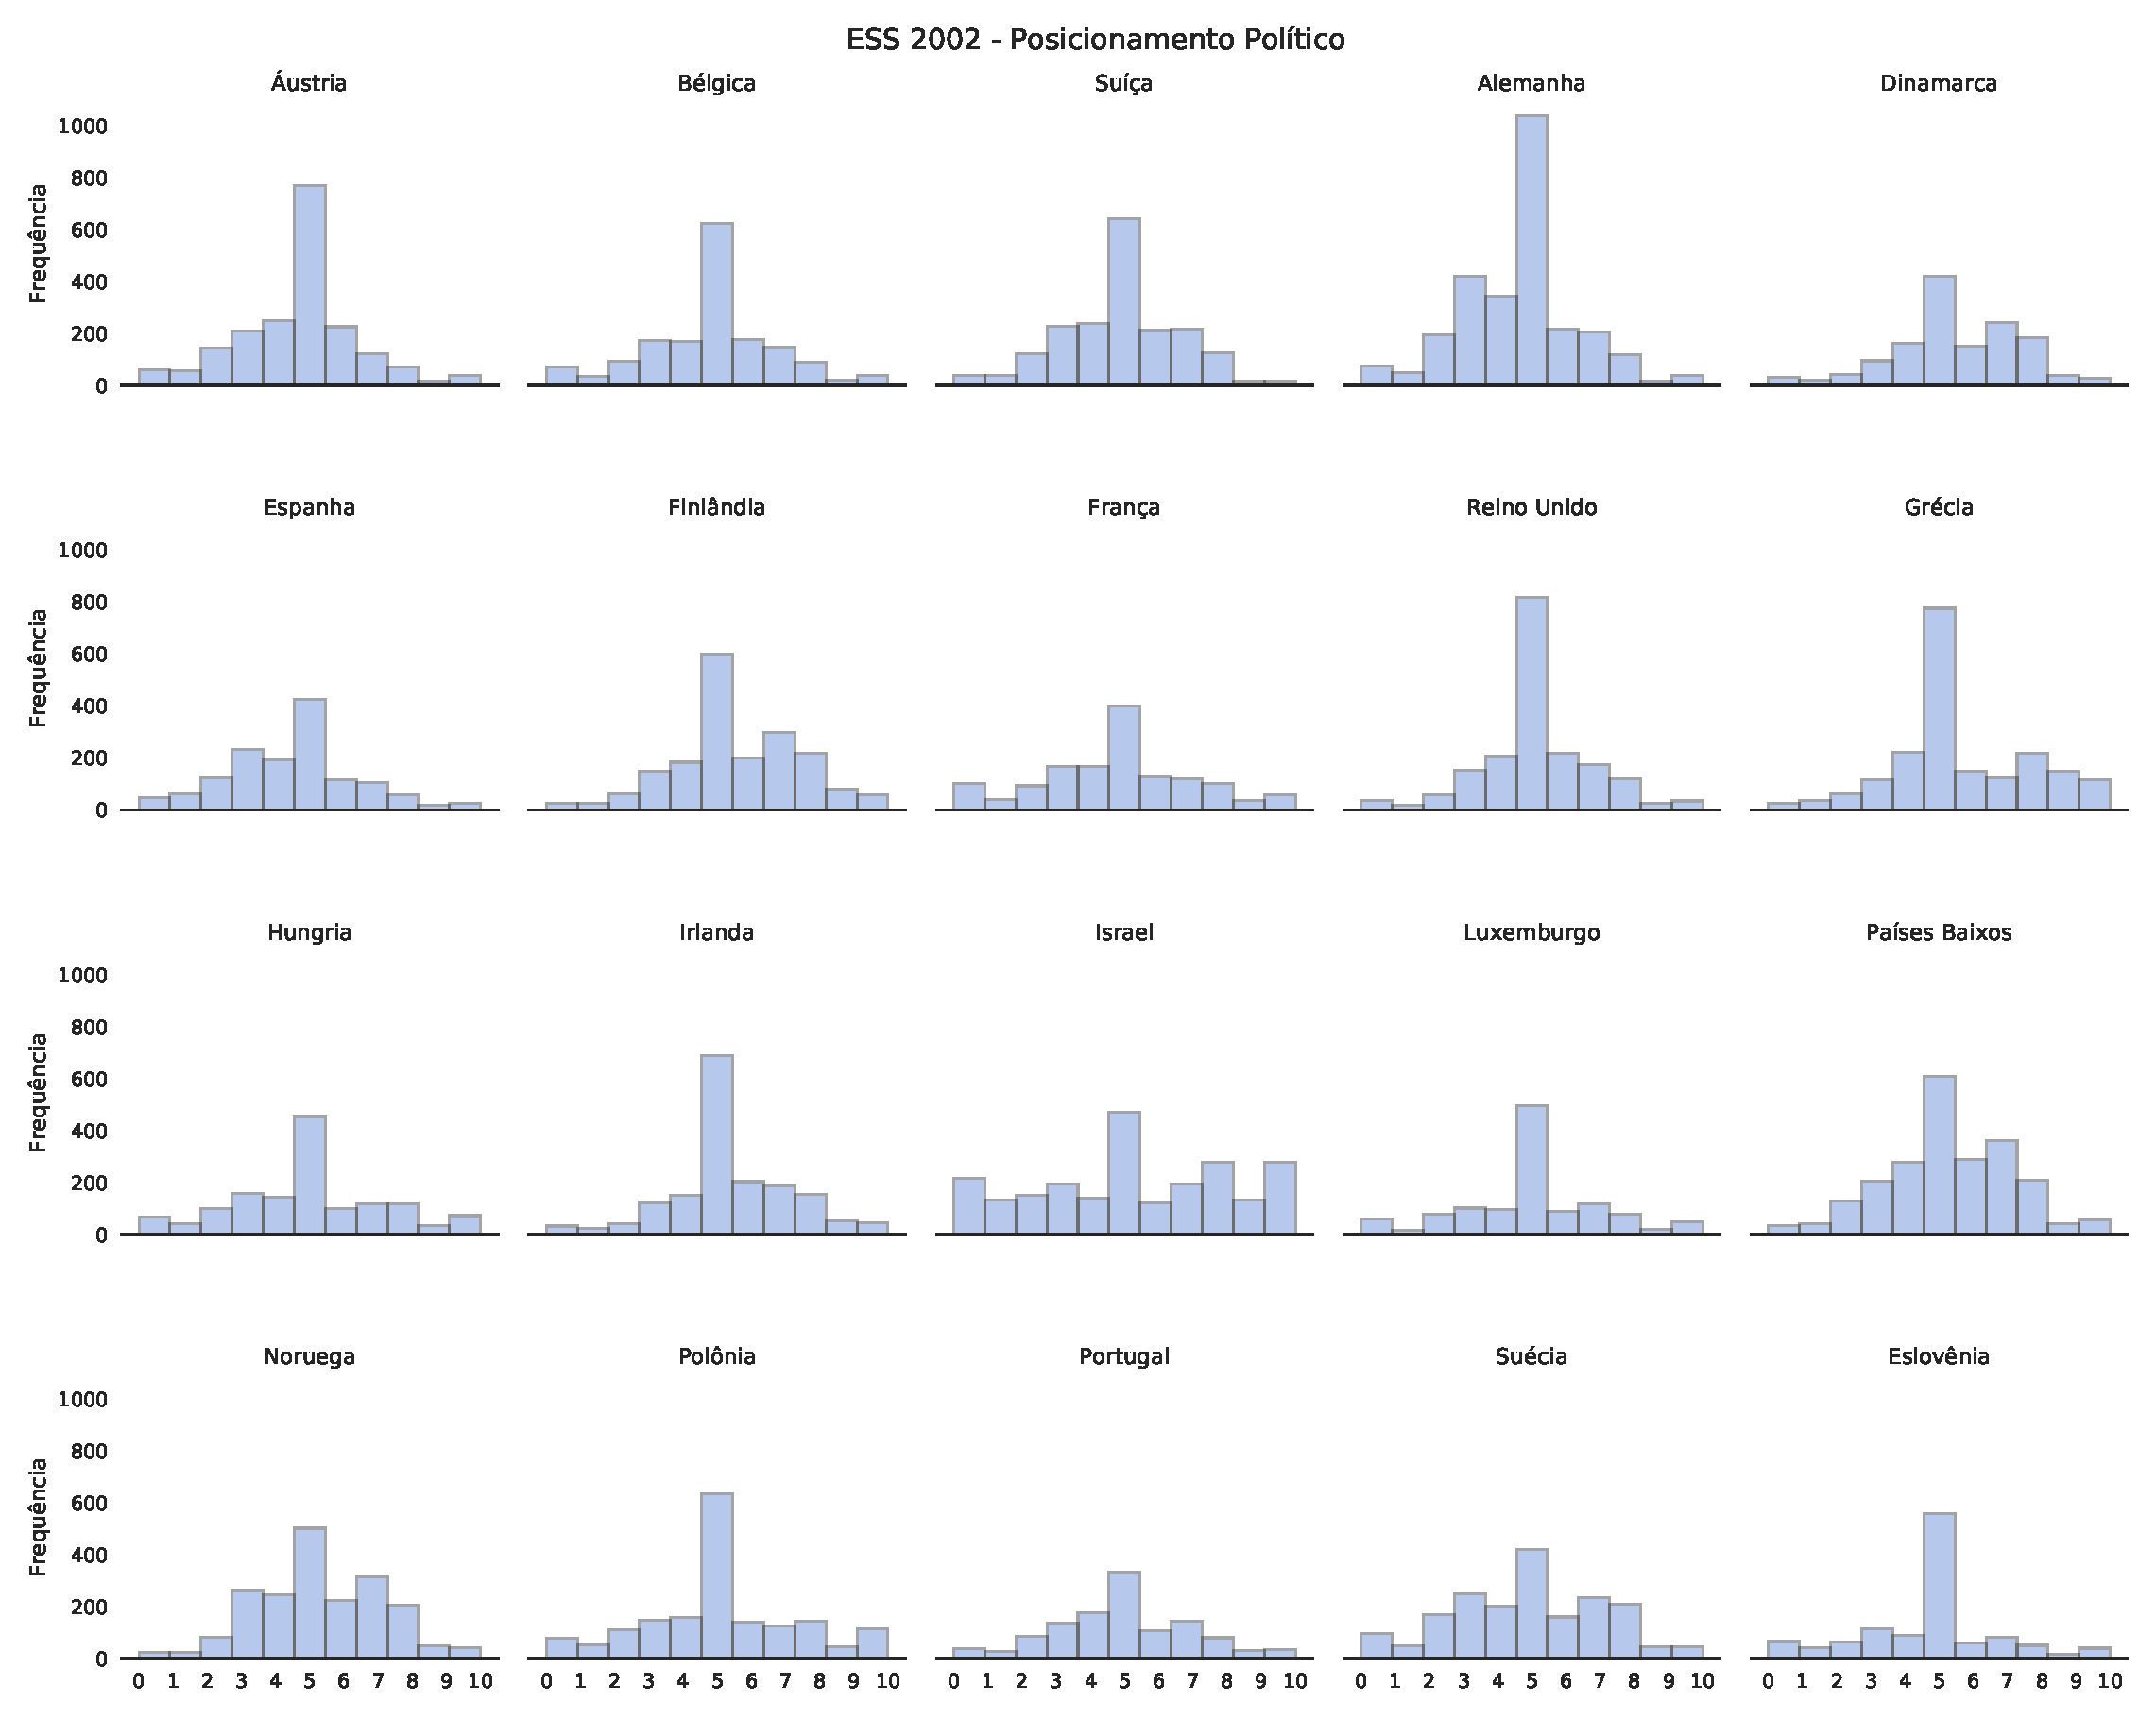
\includegraphics[scale = 0.2]{ims/ess_2002_plots.pdf}
    \caption{ Distribuição de Posicionamento Ideológico de respondentes em 20
      países}
    \label{fig2}
  \end{figure}
\end{frame}


\begin{frame}{Dinâmicas de Opinião}
  \begin{itemize}
  \item Definição de OD;
  
  \item Estrutura de um modelo de OD:
    \begin{itemize}
    \item Os agentes têm as seguintes propriedades:

      \begin{itemize}
      \item Opinião;
      \item Estrutura de Interação (topologia + regra de interação);
      \item Regra de Atualização;
      \end{itemize}
    \item Três classes \cite{flache2017}:
      \begin{itemize}
      \item Modelos de Influência Social Assimilativa;
      \item Modelos com influência enviesada  \(\leftarrow\) viés partidário;
      \item Modelos de influência repulsiva.
      \end{itemize}
      
    \end{itemize}
  \end{itemize}
\end{frame}

\begin{frame}{Modelos Canônicos em OD}
  \begin{itemize}
  \item Inspirado em Ising;
  \item Voter;
  \item Regra da Maioria;
  \item Sznajd;
  \item \textbf{Axelrod}
  \item \textbf{Deffuant-Weisbuch}
  \end{itemize}
\end{frame}

\begin{frame}{OD e Espectro Cognitivo }
  \begin{itemize}
  \item Arquiteturas Cognitivas \(\longleftrightarrow\) Modelos Fisicalistas
  \item Arquiteturas Cognitivas \(\rightarrow\) ``Maldição da Dimensionalidade''
    \cite{de2005computational}
  \item Modelos Fisicalistas \(\rightarrow\) Modelagem ad-hoc
  \end{itemize}
\end{frame}

\begin{frame}{Espectro Cognitivo e Modelos Bayesianos}
  \begin{itemize}
  \item Agentes Imperfeitamente Bayesianos: ``meio termo virtuoso''
  \item Framework de \textcite{martins2012bayesian};
  \item \textcite{martins2009bayesian} aplicação para um espaço contínuo:
    \begin{itemize}
    \item    \( o_i(t+1)
    =
    p
    \frac{o_i(t) + o_j(t)}{2}
    +
    (1-p^*)o_i(t) \)
    \item \(    \sigma_i^2(t+1)
    =
    \sigma_i^2(t)
    (1 - \frac{p^*}{2})
    +
    p^*
    (1-p^*)
    (\frac{o_i(t)-o_j(t)}{2})^2\)
    \vspace{0.3cm}
    \item Onde: \(
    p^*
    =
    \frac{
      p \frac{1}{\sqrt{2 \pi} \sigma_i}
      e^{(- \frac{o_i (t) - o_j (t))^2}{2 \sigma_i^2})}
    }{
      p
      \frac{1}{\sqrt{2 \pi} \sigma_i}
    e^{(- \frac{o_i (t) - o_j (t))^2}{2 \sigma_i^2})}
    +
    (1 - p)
  }
  \) 
  \end{itemize}
  \end{itemize}
\end{frame}

\begin{frame}{OD : Microfundamentos II}
  \begin{itemize}
  \item Regra de Interação: \(ij\);
  \item Regra de Atualização : assimilação enviesada imperfeitamente bayesiana
    (viés partidário);
  \end{itemize}
\end{frame}

\section{Modelo, Metodologia de Análise e Resultados}
\begin{frame}{Modelo}
  \begin{itemize}
  \item Atributos dos agentes:
    \begin{itemize}
    \item Perfil ideológico: \( I_i = ((o_{i,1},\sigma), \ldots,
      (o_{i,n}, \sigma) )\)
    \item Posicionamento (ponto ideal):  \(x_i = \frac{1}{n}\sum_{k=1}^{n}
      o_k\)
      \item \textcolor{gray!70}{vizinhos}
    \end{itemize}
  \end{itemize}
\end{frame}

\begin{frame}{Modelo}
  \begin{itemize}
  \item Origem de \(\sigma\) e \(o\)?
    \begin{itemize}
    \item \(\sigma\) global (parâmetro);
      \begin{itemize}
      \item Alguns agentes são ``intransigentes'' : \(\sigma \approx 0\)
      \end{itemize}
    \item Os \(o_{ik}\) são retirados de distribuições Beta (uma para cada agente)
    \end{itemize}
  \end{itemize}
\end{frame}

\begin{frame}
      
\begin{figure}[H]
  \centering
\caption{Distribuições Beta para 50 agentes}
  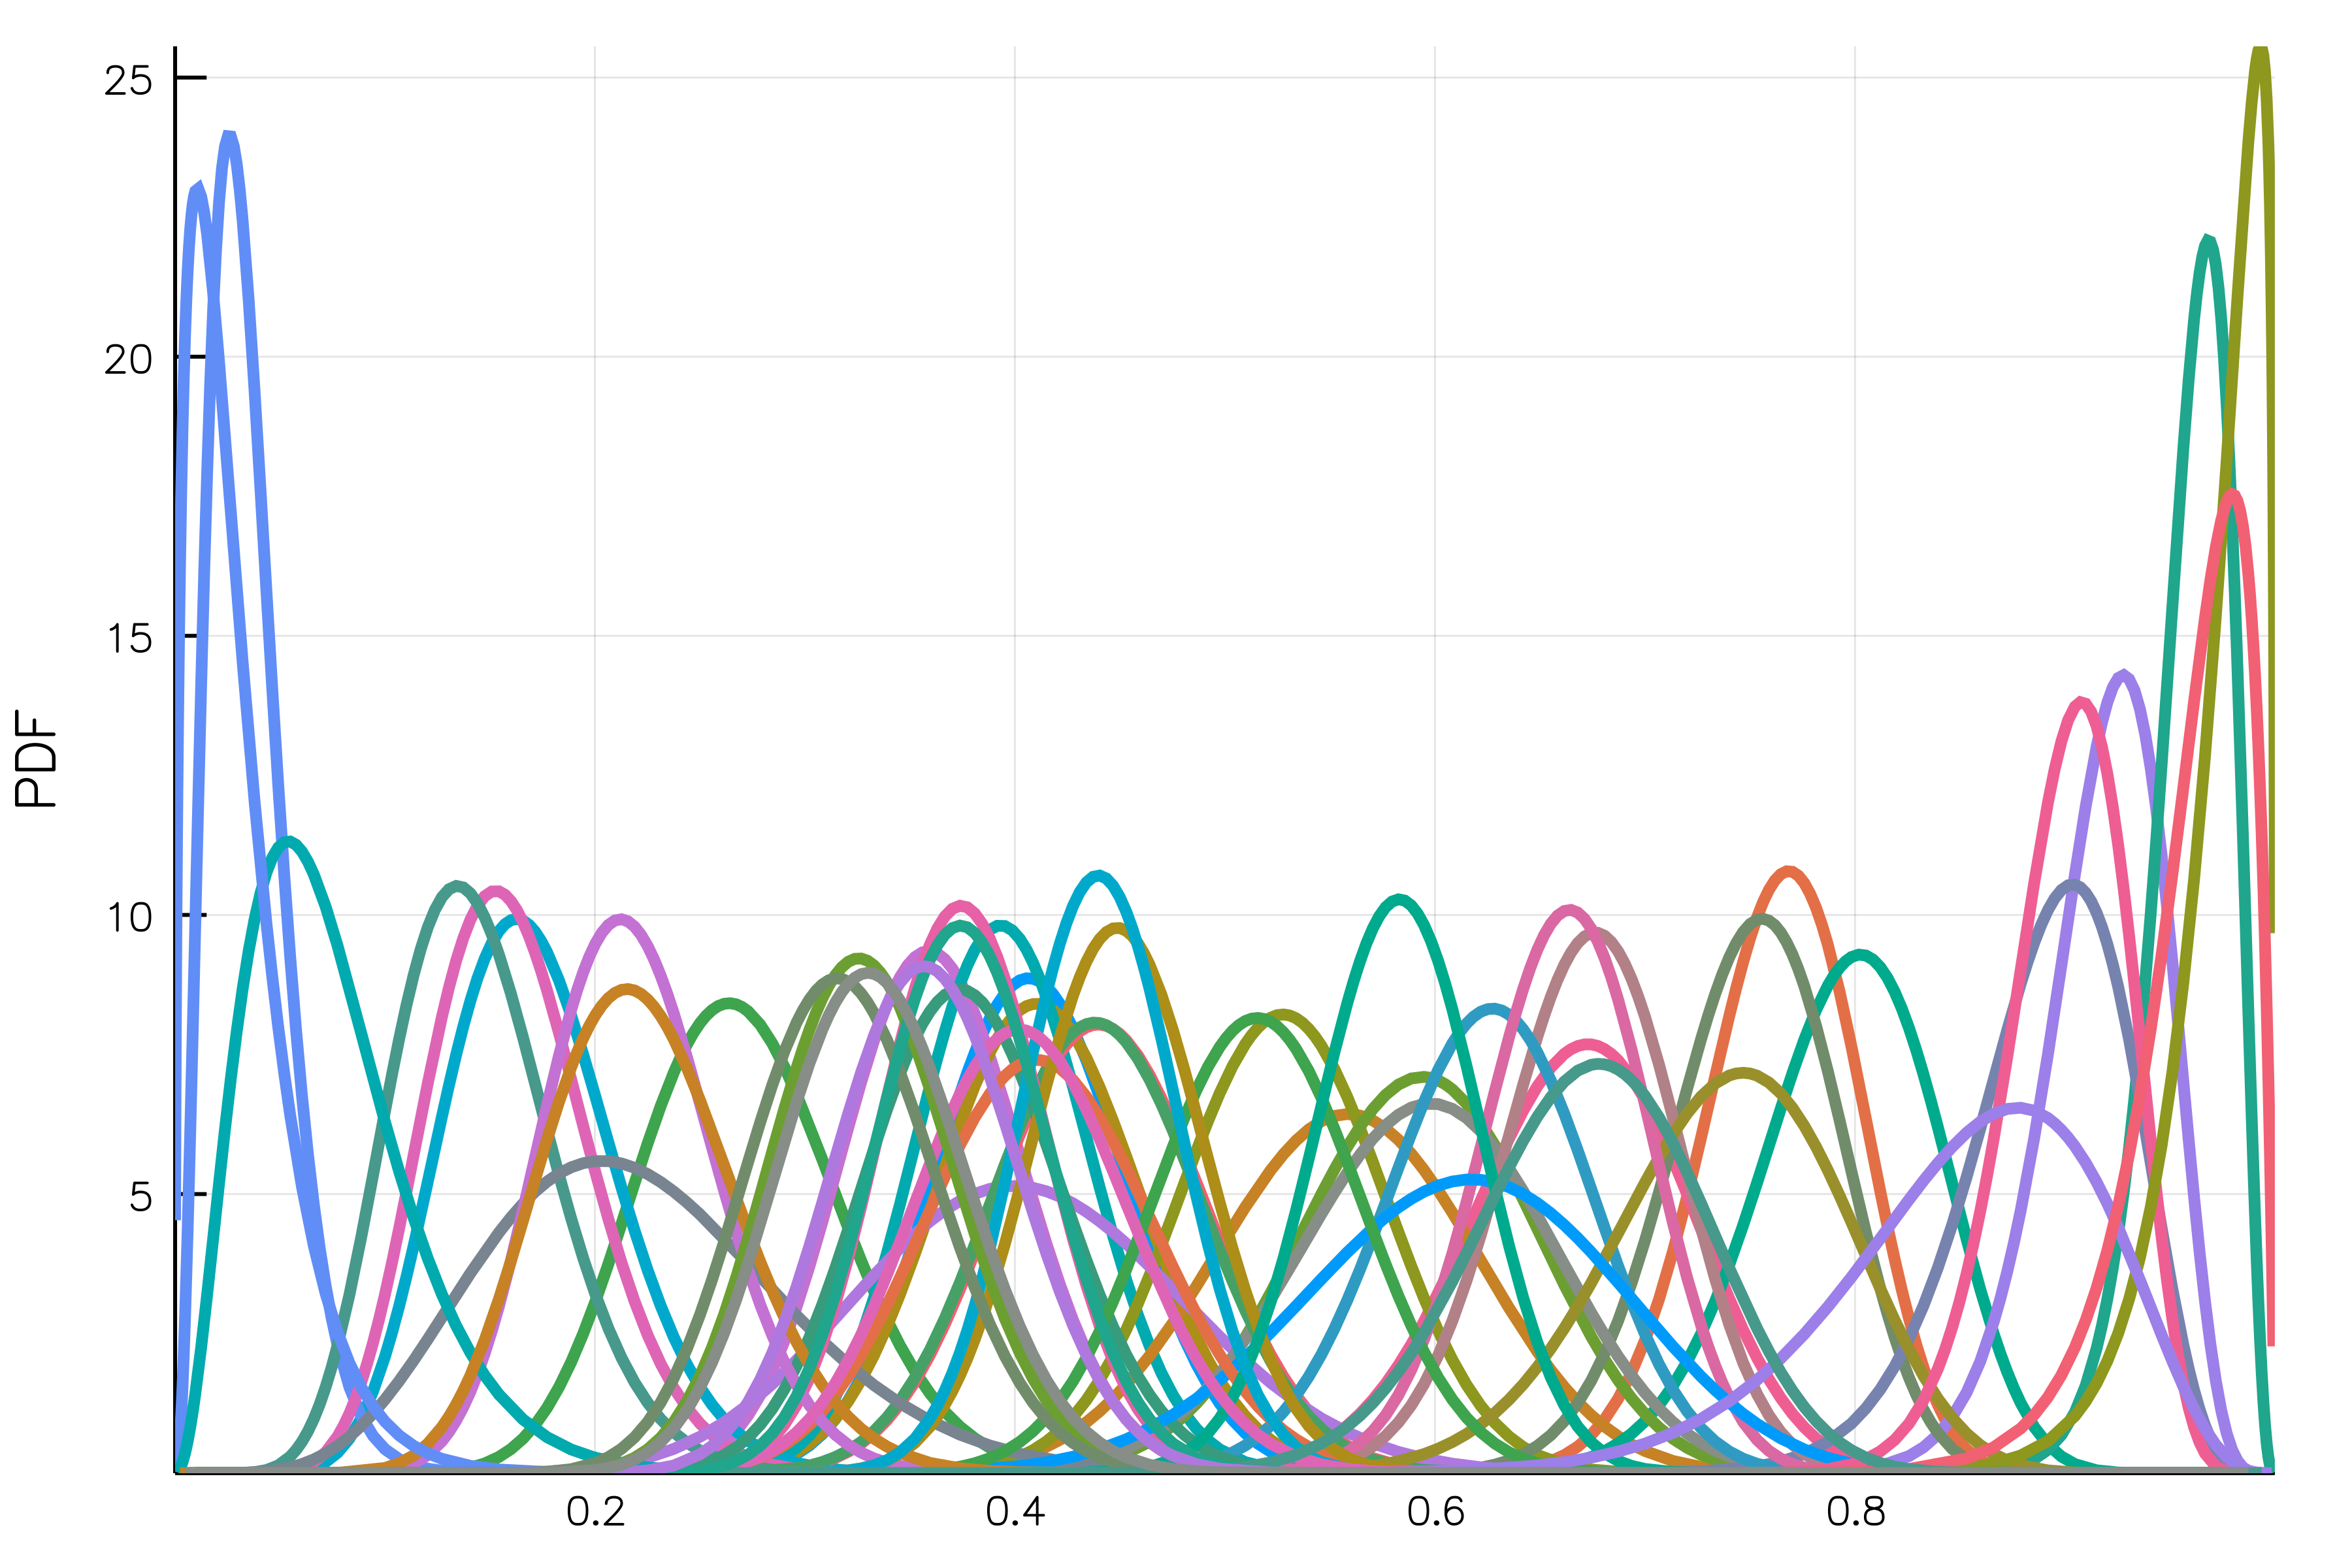
\includegraphics[scale = 0.08]{ims/beta100.png}
  \label{fig:betas100}
\end{figure}
\end{frame}

    \begin{frame}{Modelo}
      \begin{itemize}
      \item A regra de interação é entre pares;
      \item A regra de atualização é a mesma que \textcite{martins2009bayesian}:
        a cada interação o agente \(i\) atualiza  \textit{um} de seus \(o\)
        segundo \( o_i(t+1) = p \frac{o_i(t) + o_j(t)}{2} + (1-p^*)o_i(t) \)
      \item Há também ruído: \(o_i(t+1) = o_i(t) + r\) onde \(r\) é sorteado de
        uma N(0, \(\rho \))
  \end{itemize}
\end{frame}

\begin{frame}{Implementação}

Os parâmetros-chave para configuração do modelo são:
\begin{itemize}
\item A população de \(500 \leq N \leq 5.000 \) agentes;
\item O número de questões \(1 \leq n \leq 10\); 
\item As incertezas \(0.01 \leq \sigma_i \leq 0.5\);
  \begin{itemize}
  \item A incerteza é, na condição inicial, a mesma para todos os agentes;
  \item Alguns agentes têm um dos \(\sigma = 1e-20\). Qual a proporção de
    agentes intransigentes é dado pelo parâmetro: \( 0.0 \leq p\_intran \leq
    0.1\)
  \end{itemize}
  
\item O parâmetro de confiança \(0.1 \leq p \leq 0.99\);  
\item A probabilidade de reconsideração \(0.0 \leq \rho  \leq 0.1\);
  \begin{itemize}
  \item Se \(o(t) + r > 1\) então \(o(t+1) = 1\);
  \item Se \(o(t) + r < 0\) então \(o(t+1) = 0\).
  \end{itemize}
\end{itemize}
\end{frame}


\begin{frame}{Metodologia de Análise}
  \begin{itemize}
  \item Medidas : cobertura x dispersão \cite{bramson2016disambiguation};
  \end{itemize}
\end{frame}

\begin{frame}
  \begin{figure}[h]
    \centering
      \caption{Evolução dos pontos ideais dos agentes ao longo de duas realizações.
        Parametrização: \(  N = 500, p = 0.9, \rho =  1e-5, n\_issues = 1 , p\_intra
        n= 0.0 \)}
    \begin{subfigure}[b]{0.49\textwidth}
      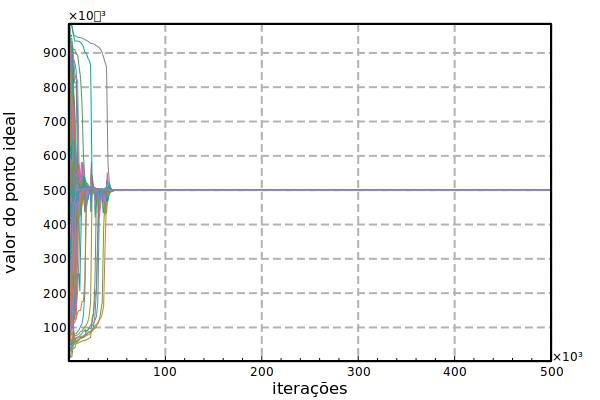
\includegraphics[width=\textwidth]{ims/timeseries1.png}
      \caption{\( \sigma = 0.1\) }
    \end{subfigure}
    \begin{subfigure}[b]{0.49\textwidth}
      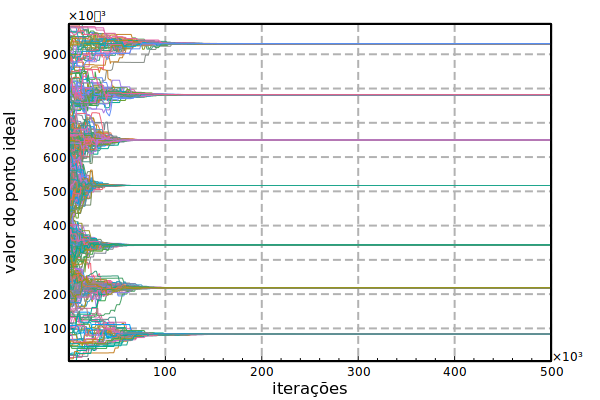
\includegraphics[width=\textwidth]{ims/timeseries2.png}
       \caption{\(\sigma = 0.02\) }
      \end{subfigure}
      
      \label{fig:tseries1}
    \end{figure}
\end{frame}

\begin{frame}
    \begin{figure}[H]
    \centering
    \caption{Parametrização equivalente a Figura \ref{fig:tseries1} (b),
      mas com \(\rho = 0.001\).}
    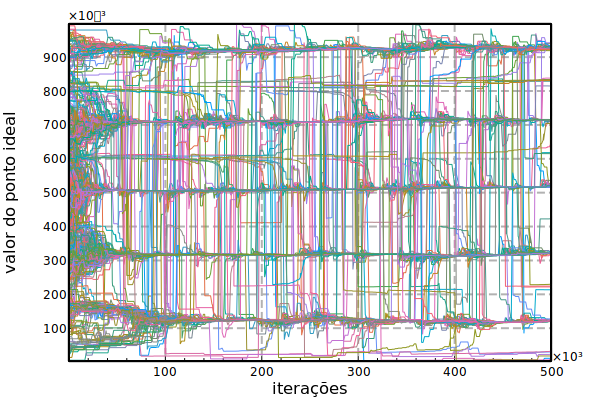
\includegraphics[width =10cm]{ims/ts5.png}
    \label{fig:nonnullrho}
  \end{figure}
\end{frame}

\begin{frame}{Metodologia de Análise}
  \begin{itemize}
  \item Output = desvio padrão dos pontos ideais;
  \item Número de iterações = 1.000.000
  \item Método de Saltelli de amostragem: n * (2d + 2) parametrizações, onde
    \(n\) é o tamanho amostral e \(d\) é o número de parâmetros \(\Rightarrow\)
    70.000 parametrizações;
  \item Índice de Sobol de sensibilidade (primeira ordem e totais)
    \cite{saltelli2008global};
  \item Gráficos de dispersão ;
    \item  Séries temporais de casos particulares.
  \end{itemize}  
\end{frame}

\begin{frame}{Resultados}
  \begin{figure}[h]
    \centering
      \caption{Desvio padrão dos pontos ideais das populações para cada
        parametrização}
    \begin{subfigure}[b]{0.49\textwidth}
      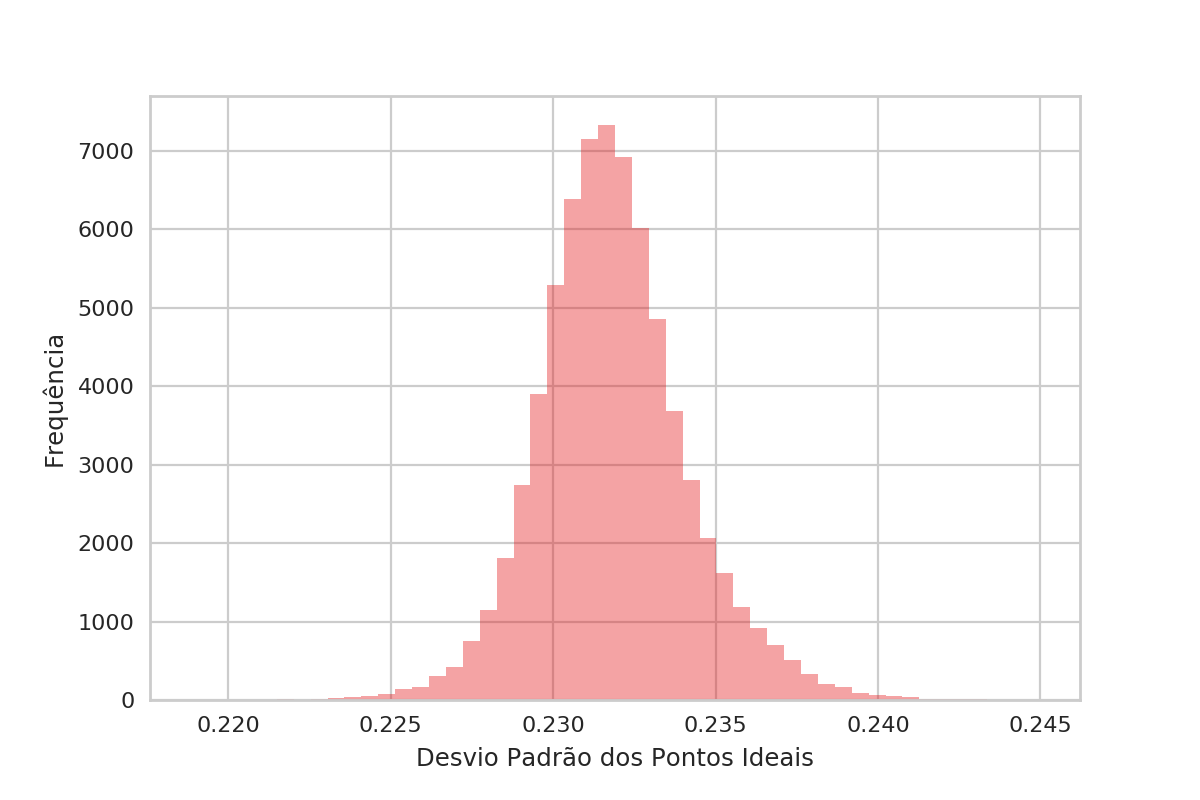
\includegraphics[width=\textwidth]{ims/diststdinit.png}
      \caption{Condição inicial}
    \end{subfigure}
    \begin{subfigure}[b]{0.49\textwidth}
      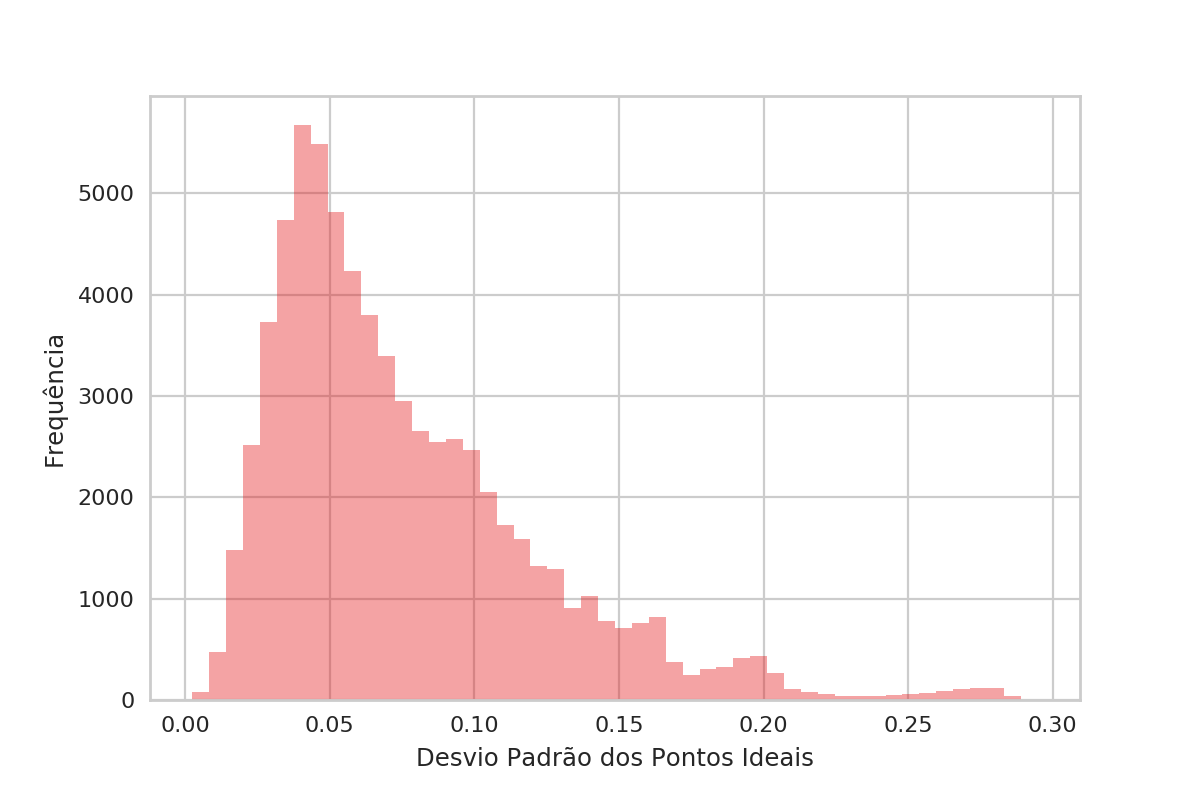
\includegraphics[width=\textwidth]{ims/distY.png}
       \caption{Após 1.000.000 iterações}
      \end{subfigure}
      \label{fig:hists1}
    \end{figure}
    
  \end{frame}
  

\begin{frame}
  \begin{figure}[H]
    \centering
    \caption{Gráfico de dispersão para 70.000 parametrizações.}
    \begin{subfigure}[b]{0.49\textwidth}
        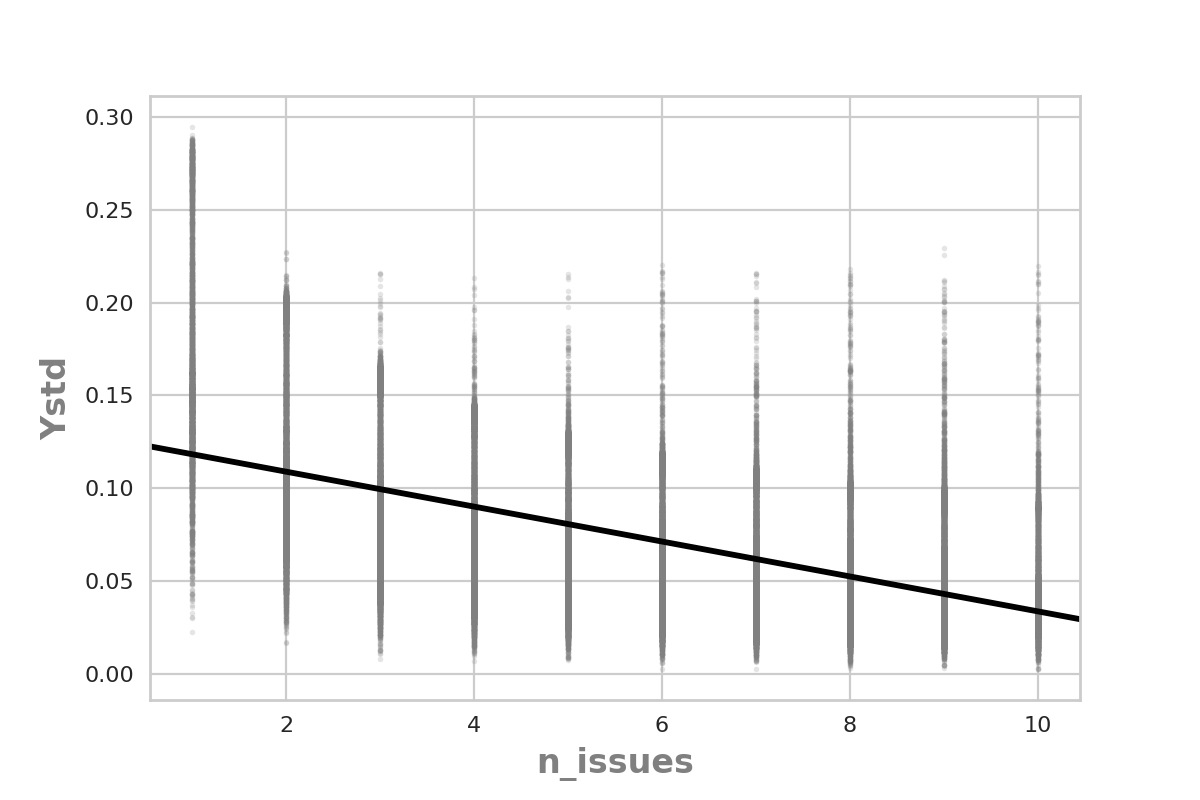
\includegraphics[width=\textwidth]{ims/mutoregressions/regressionmutatingon_issues.png}
    \end{subfigure}
    \begin{subfigure}[b]{0.49\textwidth}
        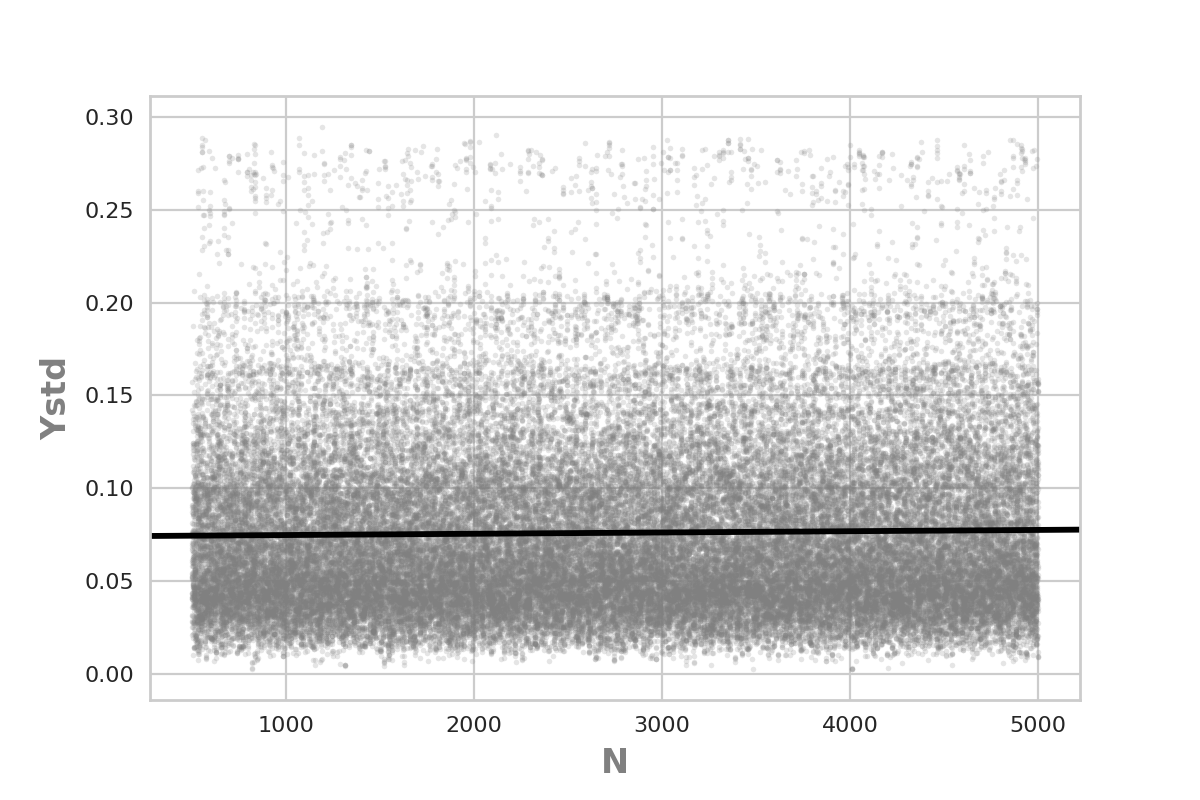
\includegraphics[width=\textwidth]{ims/mutoregressions/regressionmutatingoN.png}
    \end{subfigure}

    \begin{subfigure}[b]{0.49\textwidth}
        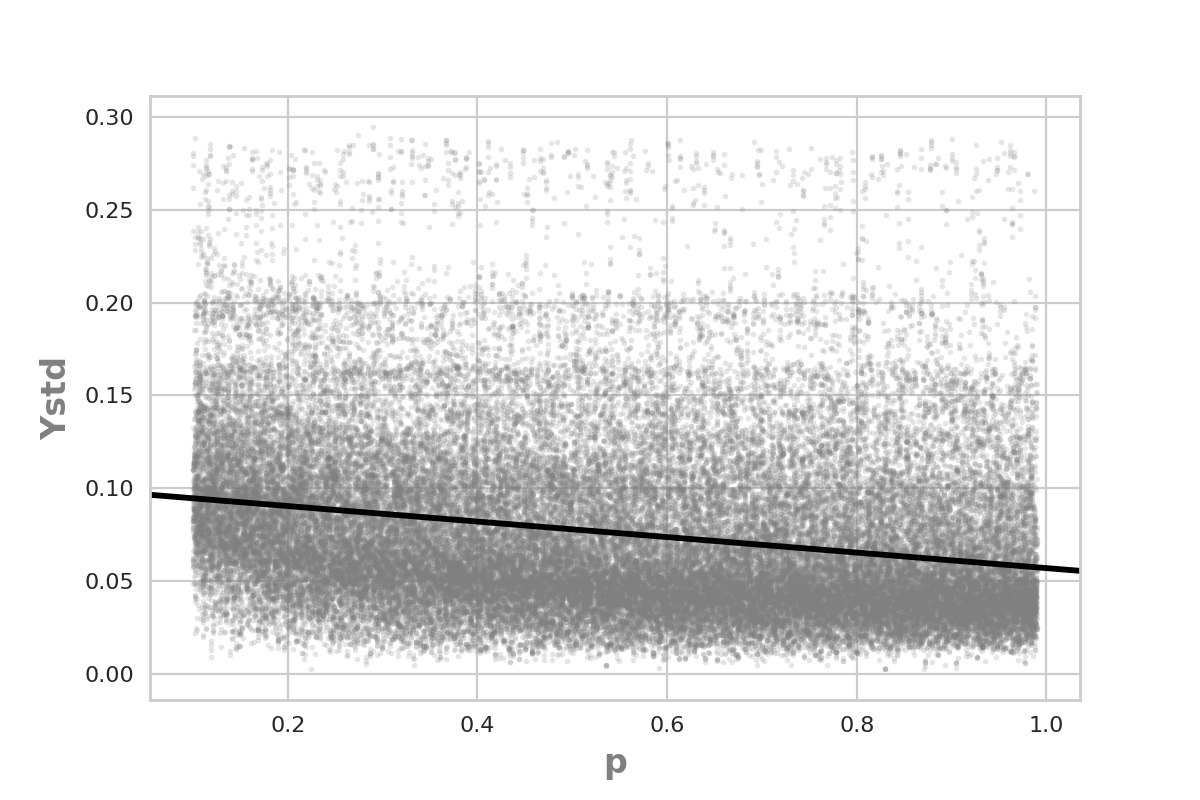
\includegraphics[width=\textwidth]{ims/mutoregressions/regressionmutatingop.png}
      \end{subfigure}
          \begin{subfigure}[b]{0.49\textwidth}
            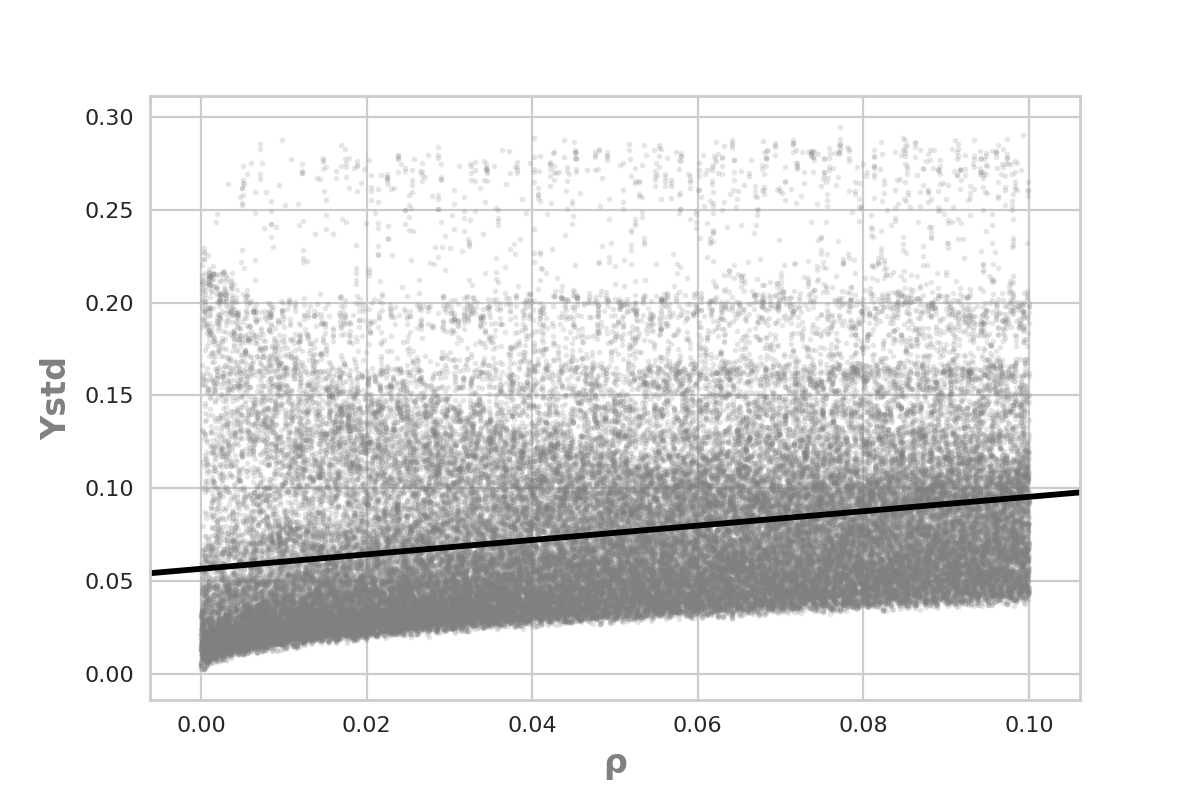
\includegraphics[width=\textwidth]{ims/mutoregressions/regressionmutatingorho.png}
      \end{subfigure}

                \begin{subfigure}[b]{0.49\textwidth}
            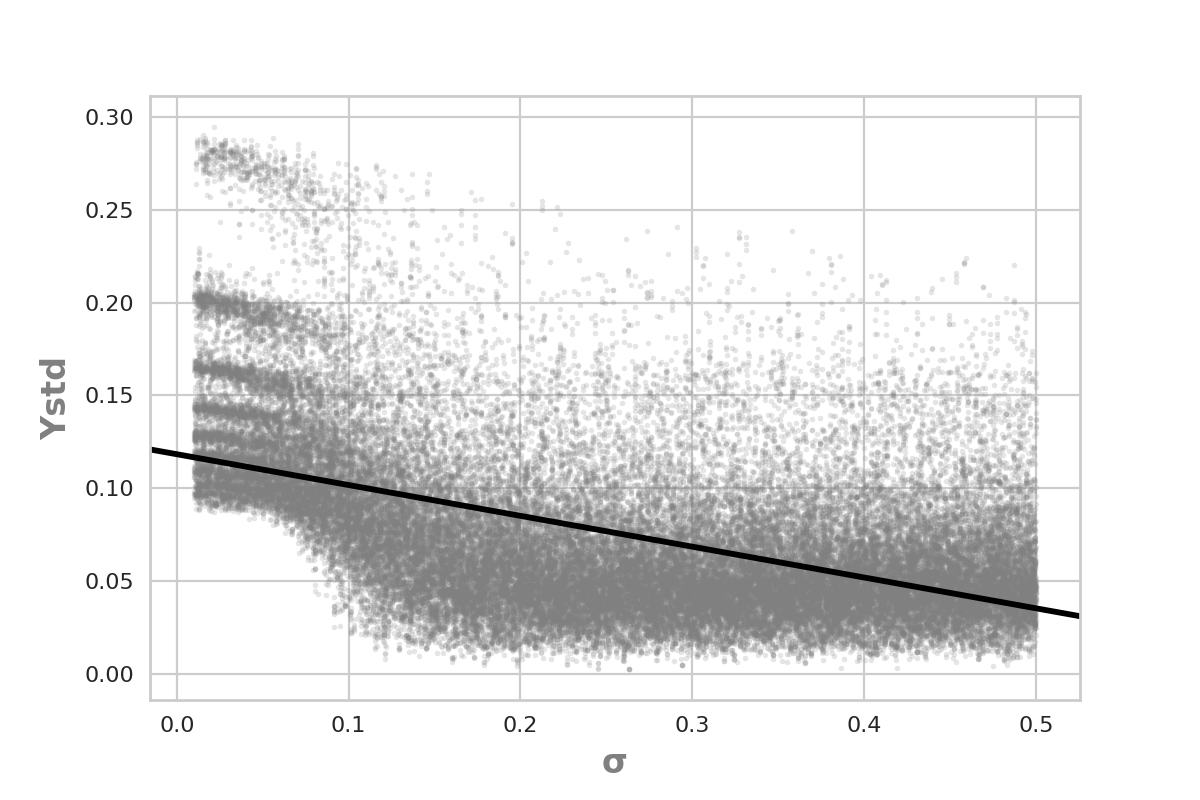
\includegraphics[width=\textwidth]{ims/mutoregressions/regressionmutatingosigma.png}
          \end{subfigure}
                \begin{subfigure}[b]{0.49\textwidth}
            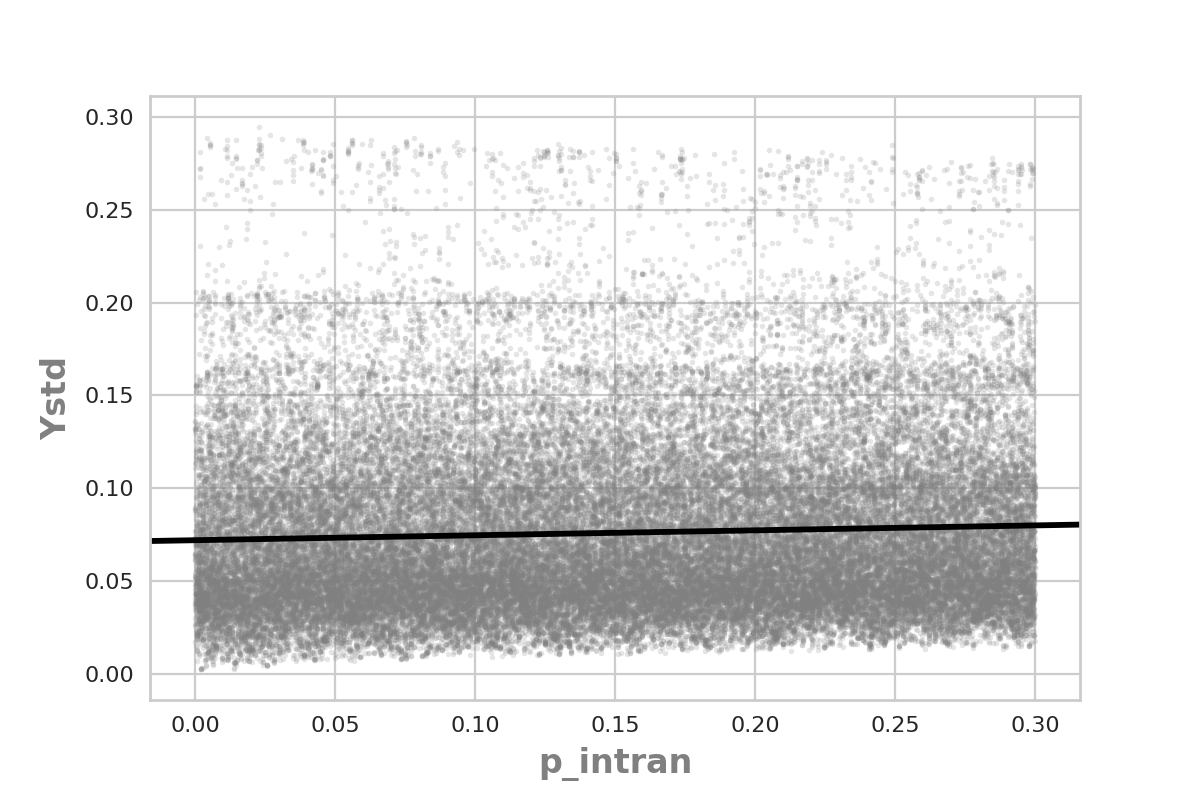
\includegraphics[width=\textwidth]{ims/mutoregressions/regressionmutatingop_intran.png}
    \end{subfigure}
    \label{fig:scatter1}
\end{figure}
\end{frame}

\begin{frame}{Resultados}  
\begin{figure}[H]
  \centering
  \caption{Índices de Sobol de sensibilidade}
  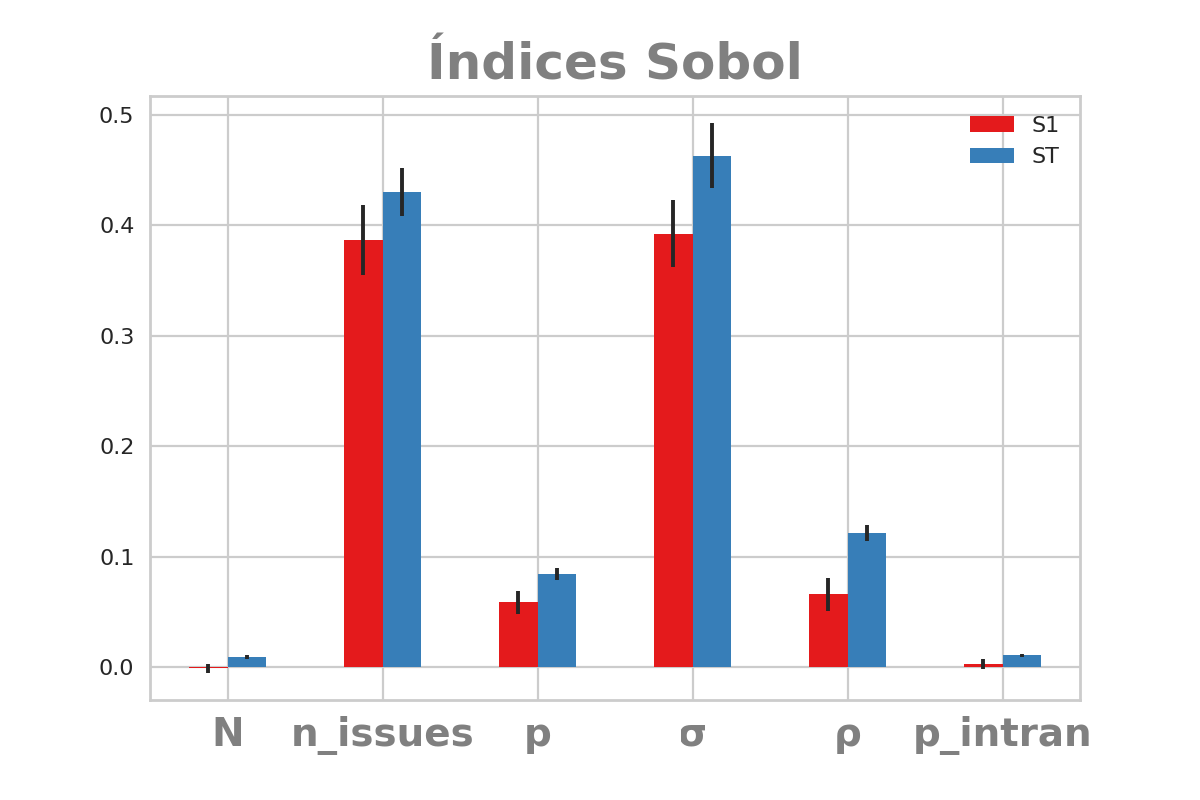
\includegraphics[scale = 0.5]{ims/barplotmuto5k.png}
  \label{fig:sobol1}
\end{figure}
\end{frame}

\begin{frame}
  \begin{figure}[H]
    \centering
      \caption{Evolução dos pontos ideais dos agentes ao longo de duas realizações.
        Parametrização: \(p\_intran = 0.15, \text{ } N = 500,  \text{ }   p =
        0.9,  \text{ }  \rho = 1e-5,  \text{ }  n\_issues = 1 \)}
    \begin{subfigure}[b]{0.49\textwidth}
      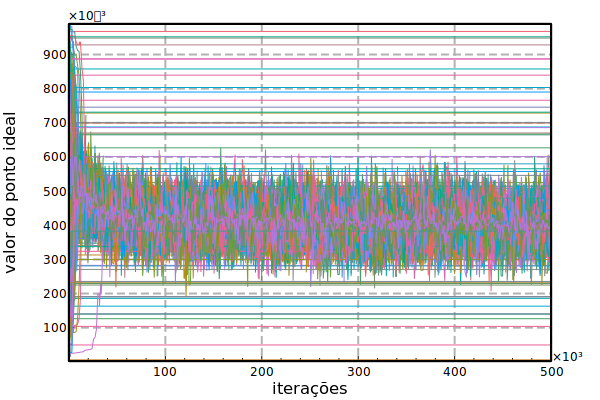
\includegraphics[width=\textwidth]{ims/timeseries3.png}
      \caption{\( \sigma = 0.1\) }
    \end{subfigure}
    \begin{subfigure}[b]{0.49\textwidth}
      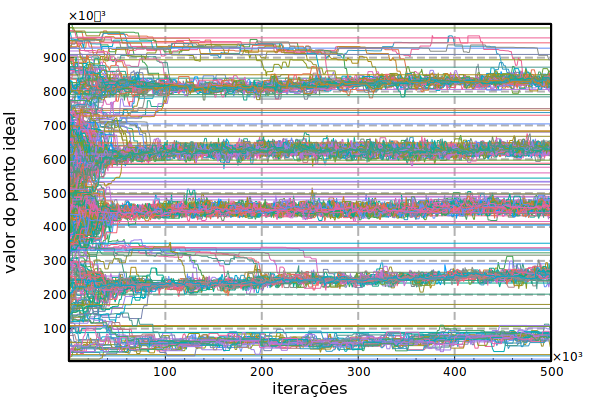
\includegraphics[width=\textwidth]{ims/timeseries4.png}
       \caption{\(\sigma = 0.02\) }
      \end{subfigure}
      \label{fig:tseries2}
    \end{figure}
\end{frame}

\begin{frame}
  
      \begin{figure}[H]
    \centering
    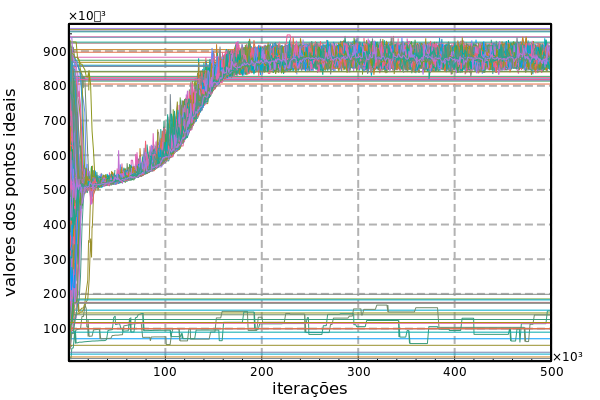
\includegraphics[scale=0.4]{ims/sigma01extremes.png}
    \caption{ Evolução dos pontos ideais dos agentes sob efeito de
      intransigentes nos extremos. Parametrização: \( \sigma = 0.1, \text{ }
      p\_intran = 0.15, \text{ } N = 500, \text{ } p = 0.9, \text{ } \rho = 1e-5,
      \text{ } n\_issues = 1 \)}
    \label{fig:tseries3}
  \end{figure}
\end{frame}

\begin{frame}
      \begin{figure}[H]
    \centering
     \caption{ Intransigentes com \(\sigma = 0.01\). Parametrização global: \( \sigma =
       0.1, \text{ } p\_intran = 0.15, \text{ } N = 500, \text{ } p = 0.9,
       \text{ } \rho = 1e-5, \text{ } n\_issues = 1 \)}
    \begin{subfigure}[b]{0.49\textwidth}
      \includegraphics[width=\textwidth]{ims/n1-sigma1.png}
      \caption{Intransigentes ideologicamente distribuídos.}
    \end{subfigure}
    \begin{subfigure}[b]{0.49\textwidth}
      \includegraphics[width=\textwidth]{ims/n1-sigma1-extremes.png}
       \caption{Itransigentes localizados nos extremos.}
     \end{subfigure}
    \label{fig:newintrans}
     \end{figure}
\end{frame}

\begin{frame}
    \begin{figure}[H]
    \centering
     \caption{ Intransigentes com \(\sigma = 0.01\). Parametrização global: \( \sigma =
       0.1, \text{ } p\_intran = 0.15, \text{ } p = 0.9,
       \text{ } \rho = 1e-5, \text{ } n\_issues = 1 \)}
    \begin{subfigure}[b]{0.3\textwidth}
      \includegraphics[width=\textwidth]{ims/sigma01_pop200.png}
      \caption{N = 200}
    \end{subfigure}
    \begin{subfigure}[b]{0.3\textwidth}
      \includegraphics[width=\textwidth]{ims/sigma01_pop700.png}
       \caption{N = 700}
     \end{subfigure}

         \begin{subfigure}[b]{0.3\textwidth}
      \includegraphics[width=\textwidth]{ims/sigma01_pop1000.png}
       \caption{N = 1000}
     \end{subfigure}
         \begin{subfigure}[b]{0.3\textwidth}
      \includegraphics[width=\textwidth]{ims/sigma01_pop1200.png}
       \caption{N = 1200}
     \end{subfigure}
    \label{fig:newintrans2}
     \end{figure}
   \end{frame}


   \begin{frame}
       \begin{figure}[H]
    \centering
    \caption{Número de pontos ideais finais para diferentes valores de \(\sigma\).
      Parametrização: \(\rho =1e-5, p\_intran = 0.0, p = 0.9, N =500\)}
    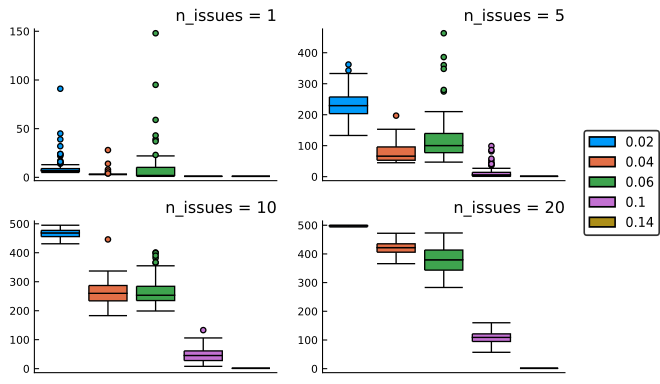
\includegraphics[scale=0.5]{ims/boxes4.png}
    \label{fig:box4}
  \end{figure}
\end{frame}

\begin{frame}
  \begin{figure}[H]
  \centering
  \caption{Evolução dos pontos ideais quando há ruído e agentes intransigentes.
        Parametrização: \(p\_intran = 0.15, \text{ } N = 500,  \text{ }   p =
        0.9,  \text{ }  \rho = 0.05\)}
    \begin{subfigure}[b]{0.3\textwidth}
      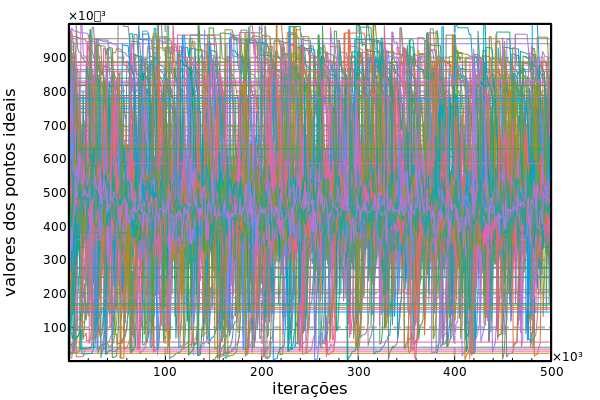
\includegraphics[width=\textwidth]{ims/n1-sigma01.png}
      \caption{\( n\_issues = 1,  \sigma = 0.1\) }
    \end{subfigure}
    \begin{subfigure}[b]{0.3\textwidth}
      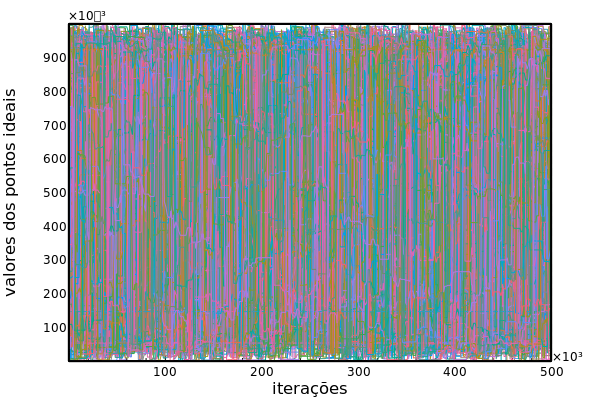
\includegraphics[width=\textwidth]{ims/n1-sigma002.png}
       \caption{\(n\_issues = 1, \sigma = 0.02\) }
     \end{subfigure}

     \begin{subfigure}[b]{0.3\textwidth}
       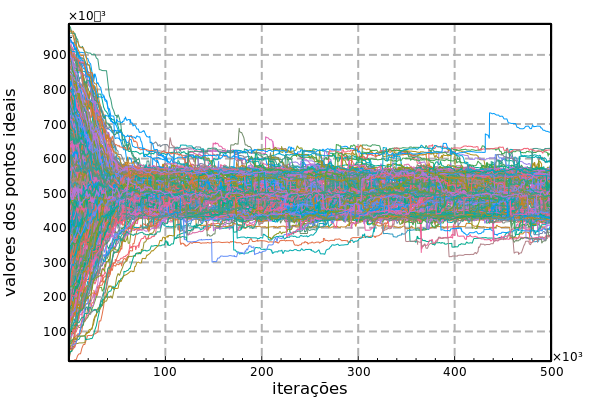
\includegraphics[width=\textwidth]{ims/n7-sigma01.png}
       \caption{\(n\_issues = 7, \sigma = 0.1\)}
     \end{subfigure}
     \begin{subfigure}[b]{0.3\textwidth}
       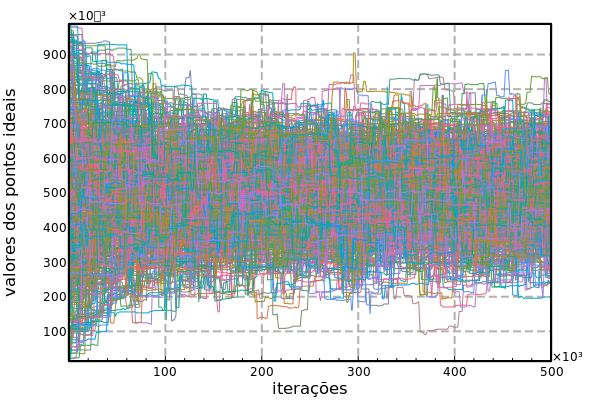
\includegraphics[width=\textwidth]{ims/n7-sigma002.png}
       \caption{\(n\_issues = 7, \sigma = 0.02\)}
     \end{subfigure}

      \label{fig:tseries4}
    \end{figure}

\end{frame}

\section{Considerações Finais}

\begin{frame}{Vindouro}
  \begin{itemize}
  \item Incorporar mídia;
  \item Testar papel da regra de interação;
  \item Testar empiricamente;
  \item Testar redes diferentes;
  \item Pensar melhor o papel do tempo;
  \end{itemize}
  
\end{frame}

\section*{Referências}
\begin{frame}[allowframebreaks]{Referências}
\printbibliography[heading=none]
\end{frame}

\end{document} 
%%% Local Variables:
%%% mode: latex
%%% TeX-master: ""
%%% End:
